 \chapter{Comparación con trabajos previos}
\doublespacing
Los antecedentes sobre la estimación del área del glaciar Quelccaya son limitados, ya que la mayoría de los estudios se han enfocado en regiones glaciares más extensas. Además, los límites glaciares utilizados en estos estudios no suelen ser consistentes, ya que los investigadores frecuentemente seleccionan manualmente las imágenes satelitales que parecen no tener nieve efímera para evitar resultados inexactos. Para comparar los resultados de esta investigación, se consideraron los estudios de \parencite{malone2022evolution}, \parencite{taylor2022multi} y \parencite{hanshaw2014glacial}. Estos estudios emplearon el método NDSI (Índice Normalizado de Diferencia de Nieve) para segmentar el glaciar Quelccaya y posteriormente estimar el área glaciar mediante un análisis temporal, usando imágenes satelitales de la serie Landsat con una resolución de 30 metros. En particular, \parencite{malone2022evolution} y \parencite{taylor2022multi} son investigaciones recientes que incluyen un análisis temporal detallado del glaciar Quelccaya.

Los resultados de la estimación de área glaciar obtenidos en este estudio presentan valores muy cercanos a los reportados en investigaciones previas. En años específicos, como 1991, 1992, 1995, 1999, 2006, 2009, 2015, 2019 y 2020, las estimaciones de área glaciar de este estudio son notablemente similares a las obtenidas en estudios anteriores. En la Figura \ref{fig:regresion_new} correspondiente, se observa que varios de estos valores se superponen o son muy cercanos a los resultados de otros estudios, aunque también existen pequeñas discrepancias. En general, los datos de este trabajo se asemejan más a los resultados de \parencite{malone2022evolution}. Sin embargo, las diferencias menores en algunos años podrían atribuirse a variaciones en la delimitación de los bordes del glaciar o a fenómenos climáticos interanuales, como El Niño o La Niña. Cabe destacar que los datos de esta investigación cuentan con una resolución espacial de 30 metros, equivalente a la de los estudios comparados.

En cuanto a los resultados específicos, para el año 1991 (inicio del análisis temporal en este estudio), la estimación del área glaciar en \parencite{taylor2022multi} fue de 50.21 km², en \parencite{malone2022evolution} fue de 50.89 km², mientras que en este estudio fue de 50.81 km². Para el año 2020, último año de análisis en \parencite{taylor2022multi} y \parencite{malone2022evolution}, los valores de área glaciar fueron 41.58 km² en \parencite{taylor2022multi}, 39.03 km² en \parencite{malone2022evolution} y 38.99 km² en este estudio. Se observa que los resultados obtenidos en esta investigación son muy similares a los de \parencite{malone2022evolution}. La tasa de retroceso glaciar estimada por \parencite{malone2022evolution} fue de 0.43 km²/año, mientras que en este estudio se obtuvo una tasa de 0.393 km²/año. Es importante señalar que \parencite{taylor2022multi} no proporciona una tasa de retroceso específica para el glaciar Quelccaya.

Este estudio amplía el análisis temporal hasta 2024, año en el cual el área glaciar se ha reducido a 35.49 km². En la Figura \ref{fig:regresion_new} correspondiente se pueden observar algunos años excluidos del análisis; esto se debe a que las imágenes de esos años presentaban nieve temporal o nubes, lo cual afectaría la precisión de los resultados. Además, algunas imágenes no estaban disponibles para todos los años, lo que limitó la continuidad en ciertas observaciones.

\begin{figure}[h!]
	\centering
	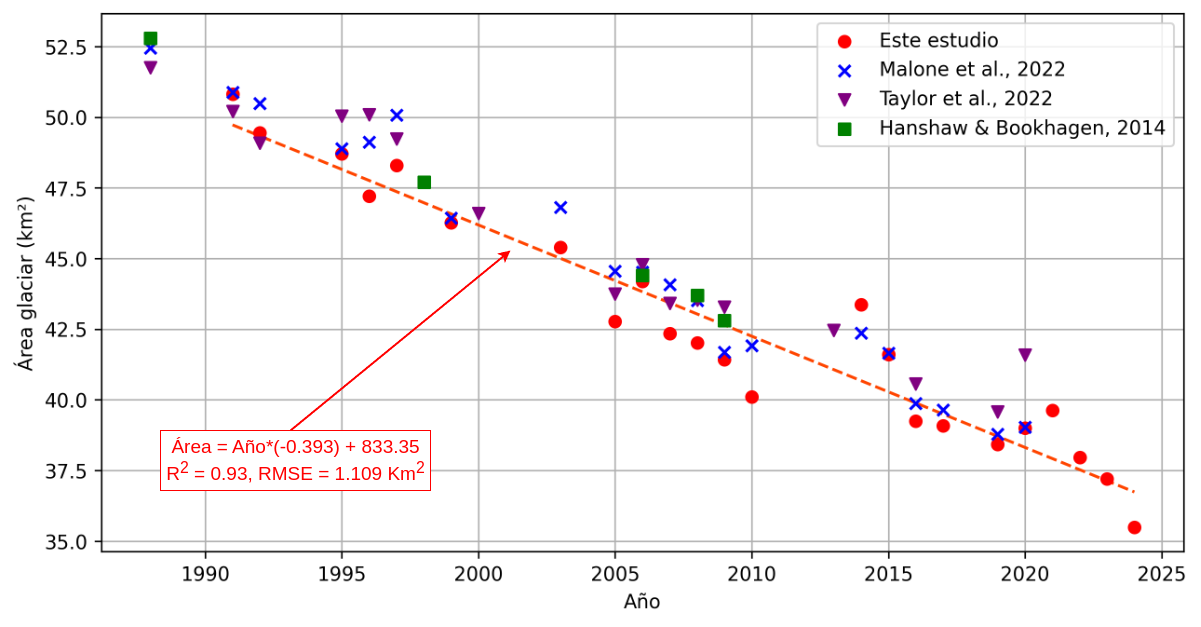
\includegraphics[width=\linewidth]{graficos/regresion_new}
	\caption[Serie temporal de superficie glaciar Quelccaya.]{Serie temporal del área glaciar del Quelccaya. Los puntos rojos representan el área glaciar estimada en cada año según los resultados de este estudio, mientras que los demás símbolos corresponden a las estimaciones de estudios previos. La línea entrecortada muestra la regresión lineal obtenida para este estudio, con un coeficiente de determinación del 93 \% y un error cuadrático medio (RMSE) de 1.109 km². Además, se destaca la tasa de retroceso de la superficie glaciar, estimada en 0.393 km²/año.
		
	}
	\label{fig:regresion_new}
\end{figure}
\singlespacing